\setlength{\columnsep}{3pt}
\begin{flushleft}
	\bigskip
	\begin{itemize}
		\item A run level defines what system services are operating in whole OS.
		\item There are total 7 run levels.
		\item Starting with RHEL 7, \textbf{run level concept is removed and is replaced with "target units"}.
		\item Below shows the list of all runlevels and their equivalent targets:
	\begin{figure}[h!]
		\centering
		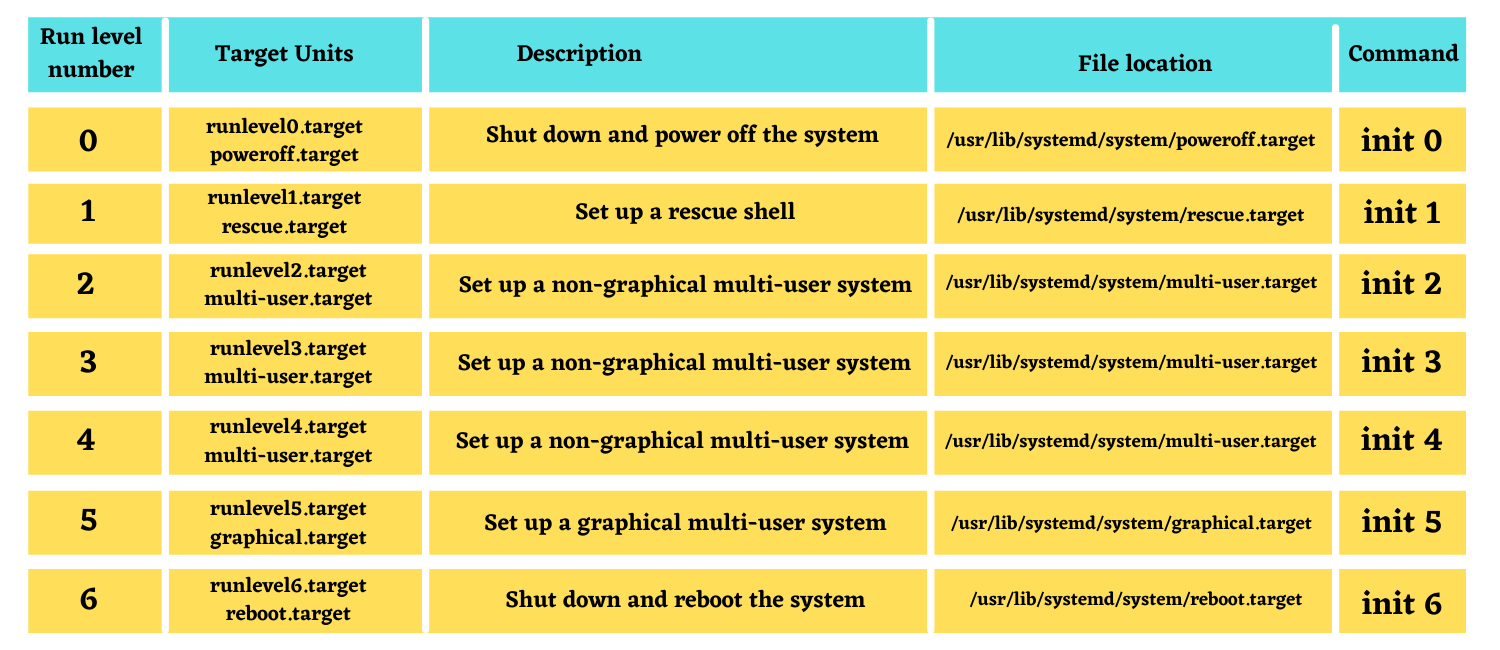
\includegraphics[scale=0.35]{content/chapter17/images/run.png}
		\caption{Targets in Linux}
		\label{fig:stage}
	\end{figure}

	\item In RHEL 8, all target unit files are stored under location \textbf{/usr/lib/systemd/system/} or \textbf{/etc/systemd/system/} and have extension \textbf{".target"}.
		

	\end{itemize}
	
	
\end{flushleft}
\newpage